\documentclass[tikz,border=10pt]{standalone}
\usetikzlibrary{arrows,intersections}
\begin{document}
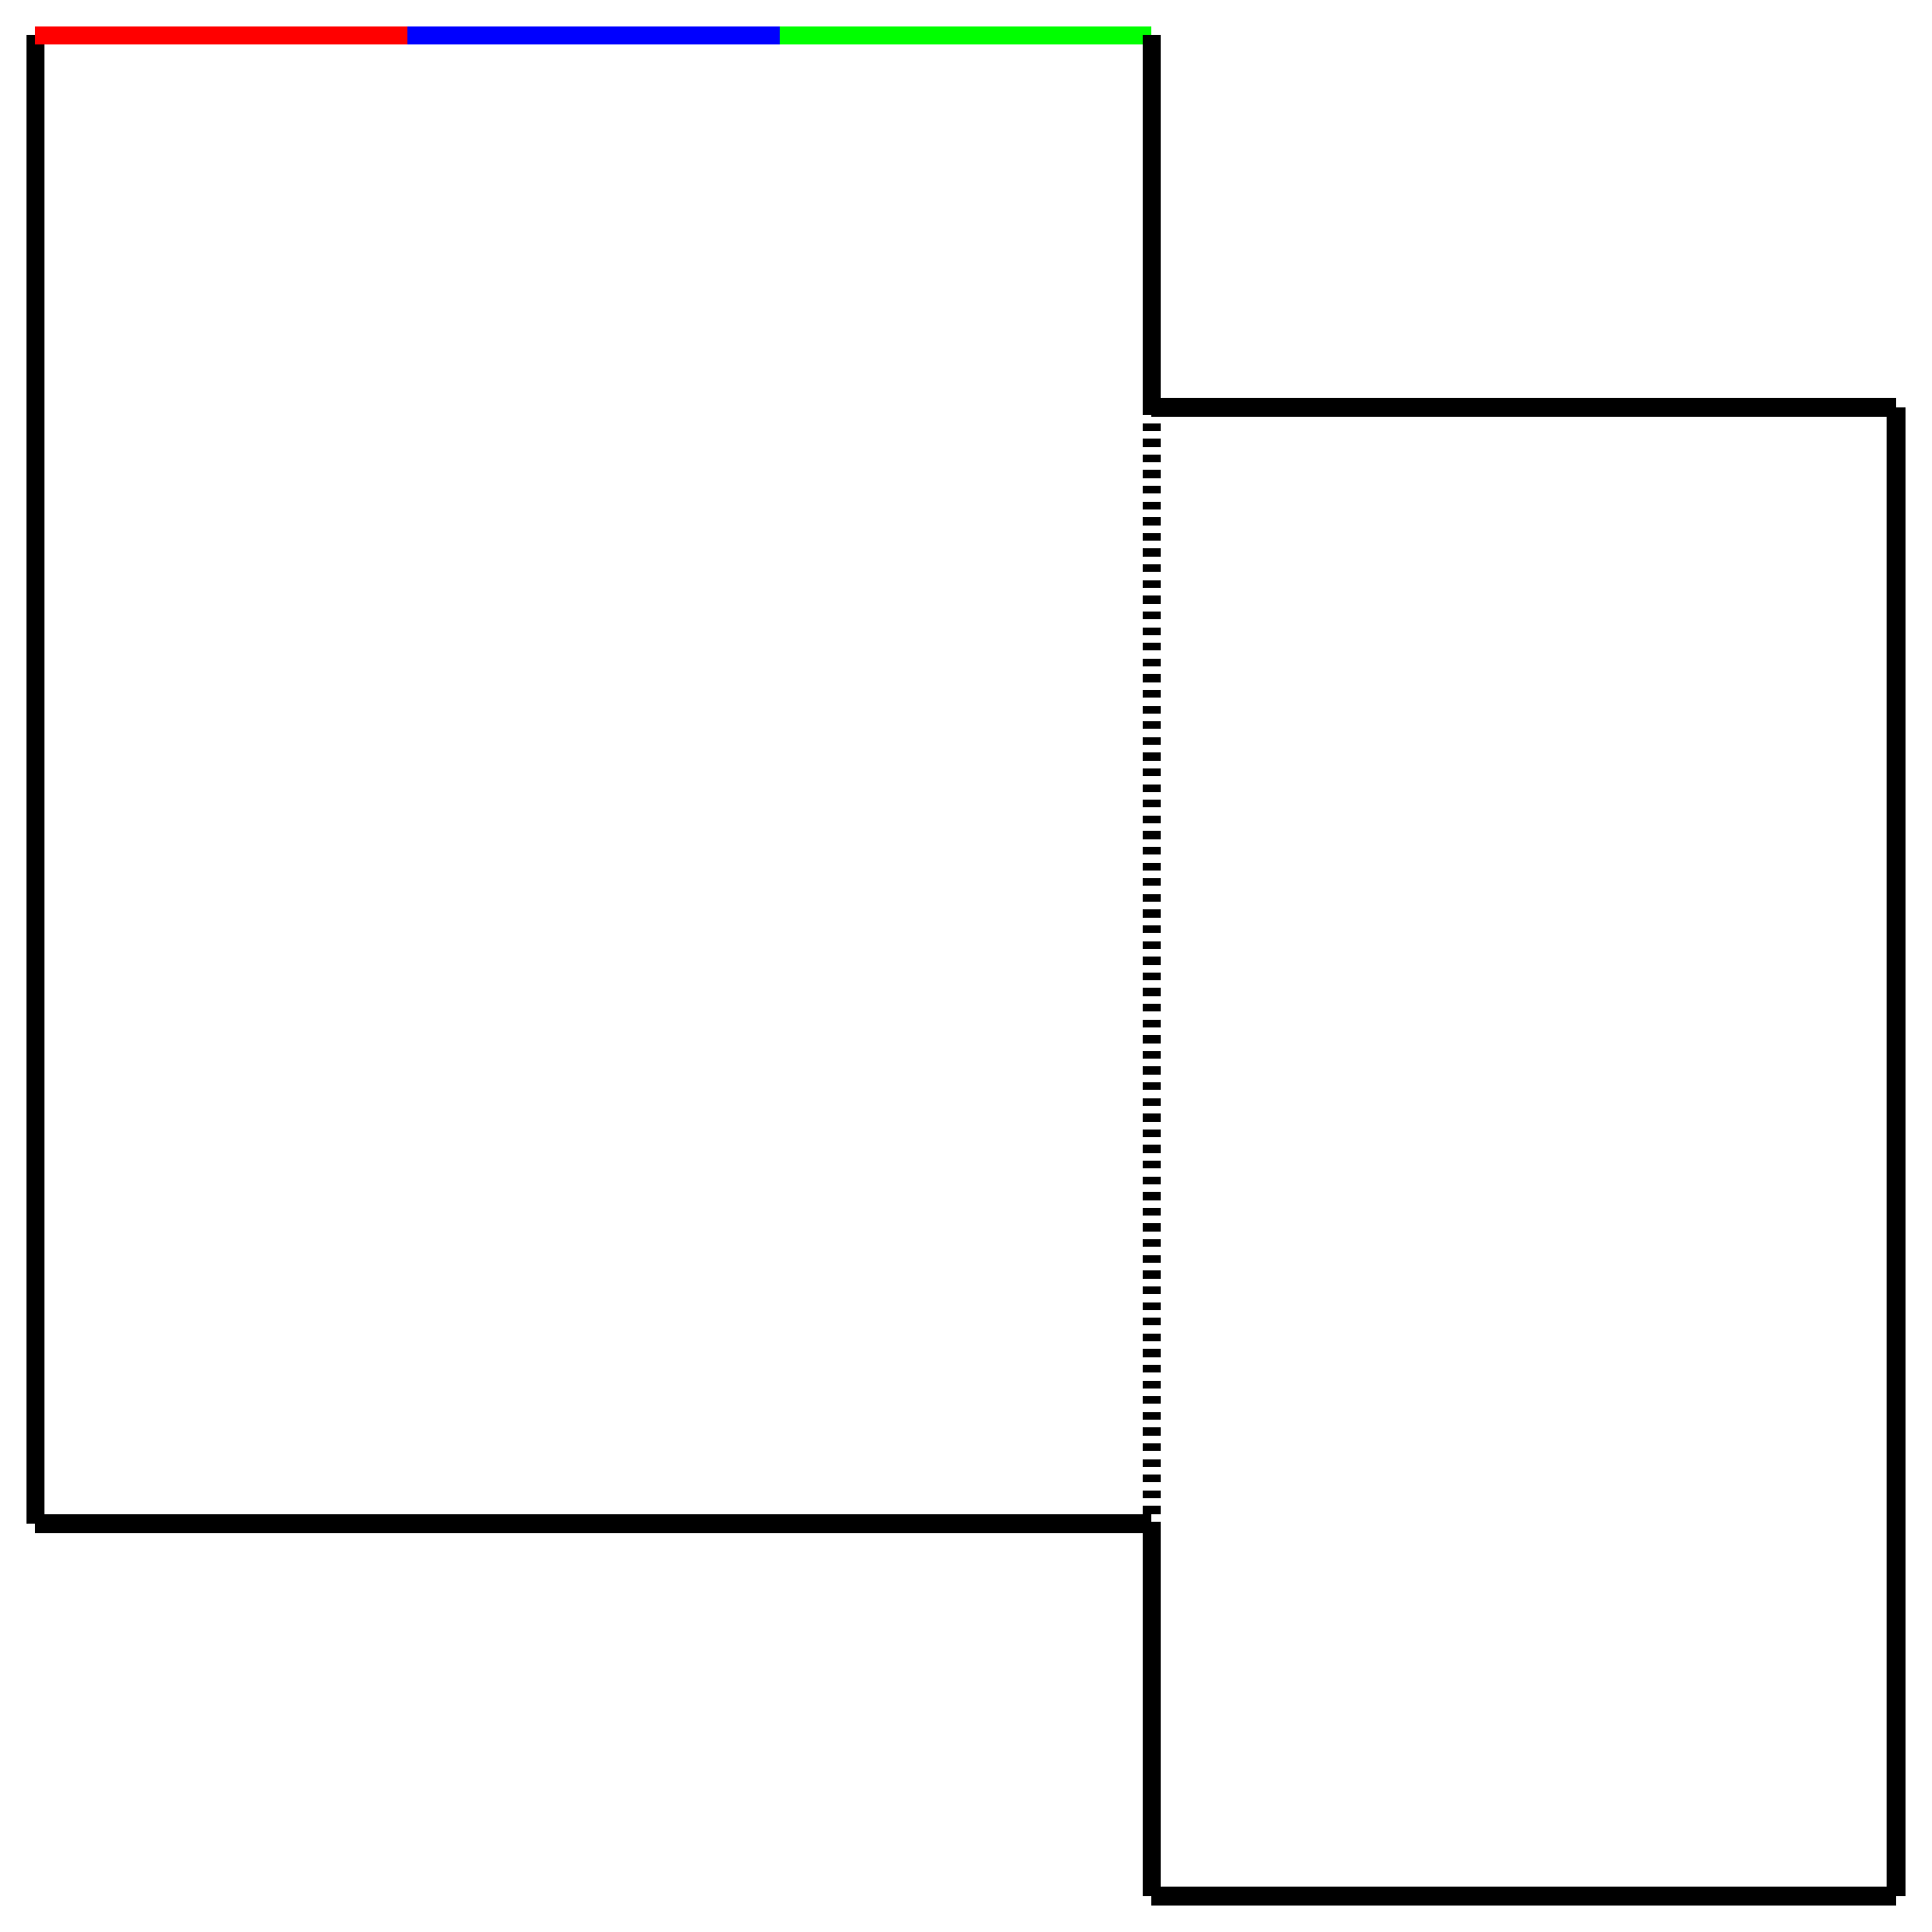
\begin{tikzpicture}[
    thick,
    >=stealth',
    dot/.style = {
      draw,
      fill = white,
      circle,
      inner sep = 0pt,
      minimum size = 4pt
    }
  ]
  \coordinate (O) at (0,0);
  \scope[]
    \draw[black, line width=7] plot[] coordinates {(0,0) (0,20)};
    \draw[red, line width=7] plot[] coordinates {(0,20) (5,20)};
    \draw[blue, line width=7] plot[] coordinates {(5,20) (10,20)};
    \draw[green, line width=7] plot[] coordinates {(10,20) (15,20)};
    
    \draw[black, line width=7] plot[] coordinates {(0,0) (15,0)};
    
    \draw[black, line width=7] plot[] coordinates {(15,20) (15,15)};
    \draw[black, line width=7, /tikz/dashed] plot[] coordinates {(15,15) (15,0)};
    
    \draw[black, line width=7] plot[] coordinates {(15,0) (15,-5)};
    \draw[black, line width=7] plot[] coordinates {(15,-5) (25,-5)};
    \draw[black, line width=7] plot[] coordinates {(25,-5) (25,15)};
    \draw[black, line width=7] plot[] coordinates {(25,15) (15,15)};
    
  \endscope
\end{tikzpicture}
\end{document}